\documentclass[9pt,twocolumn,twoside]{fernandes_paper} 
%Default opts:9pt,twocolumn,twoside
\graphicspath{{images_paper/}}

\newcommand{\mf}[1]{\colorbox{blue!10}{\color{color3}#1}}

\title{Utilizing Design Principles from Glass Sponges for Structurally Robust Lattices}

\author[1]{Matheus C. Fernandes}
\author[2]{James C. Weaver}
\author[1,3,*]{Katia Bertoldi}

\affil[1]{John A. Paulson School of Engineering and Applied Sciences -- Harvard University, Cambridge, MA 02138}
\affil[2]{Wyss Institute -- Harvard University, Cambridge, MA 02138}
\affil[3]{Kavli Institute -- Harvard University, Cambridge, MA 02138}
\affil[*]{Corresponding author: \href{mailto:bertoldi@seas.harvard.edu}{bertoldi@seas.harvard.edu}}

\keywords{Architected materials, truss structure, buckling resistance, glass sponges, bio-inspired engineering.}

\usepackage{comment}

\begin{document}
\maketitle
% \doublespace
%\linenumbers

\section{Introduction}
\subsection{Sponge Biology}
\subsection{History of Diagonally Reinforced Structures and Previous Works}
\subsection{Examples of Current Diagonally Reinforced Designs}

\section{Methods}
\subsection{Numerical Model Setup}
\subsection{Experimental Design}

\section{Results}
\subsection{Linear Stiffness for different Designs}
 \subsection{Buckling Resistance for Different Designs}
\subsection{Experimental Results}

\section{Discussion}
\subsection{Parameter Exploration}
\subsection{Parameter Optimization}

\section{Conclusion}

\section*{Acknowledgments}
\section*{References}

\begin{figure*}[ht]
  \captionsetup{width=0.8\textwidth}
\begin{center}
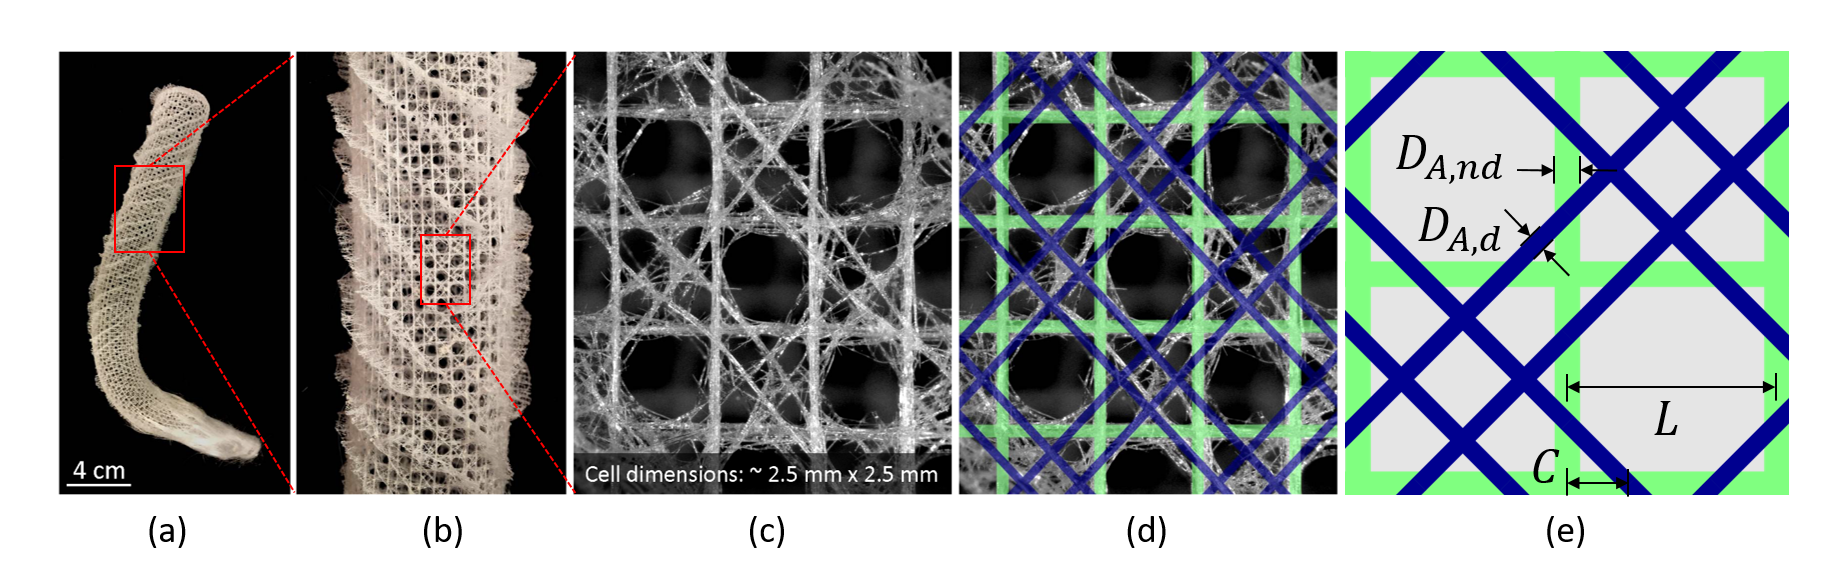
\includegraphics[width=0.9\textwidth]{Fig1}
\end{center}
\caption{\textbf{Hexactinellid sponge \textit{Euplectella aspergillum.}} (a)-(b) Full-frame photo of sponge. (c) Close up microscope image of the sponge. (d) Comparison between the idealized model (green and blue lines) and the sponge structure. (e) Representative volume element unit cell of the idealized model.}\label{Fig1}
\end{figure*}

\begin{figure*}[ht]
	\centering
	\captionsetup{width=0.8\textwidth}
	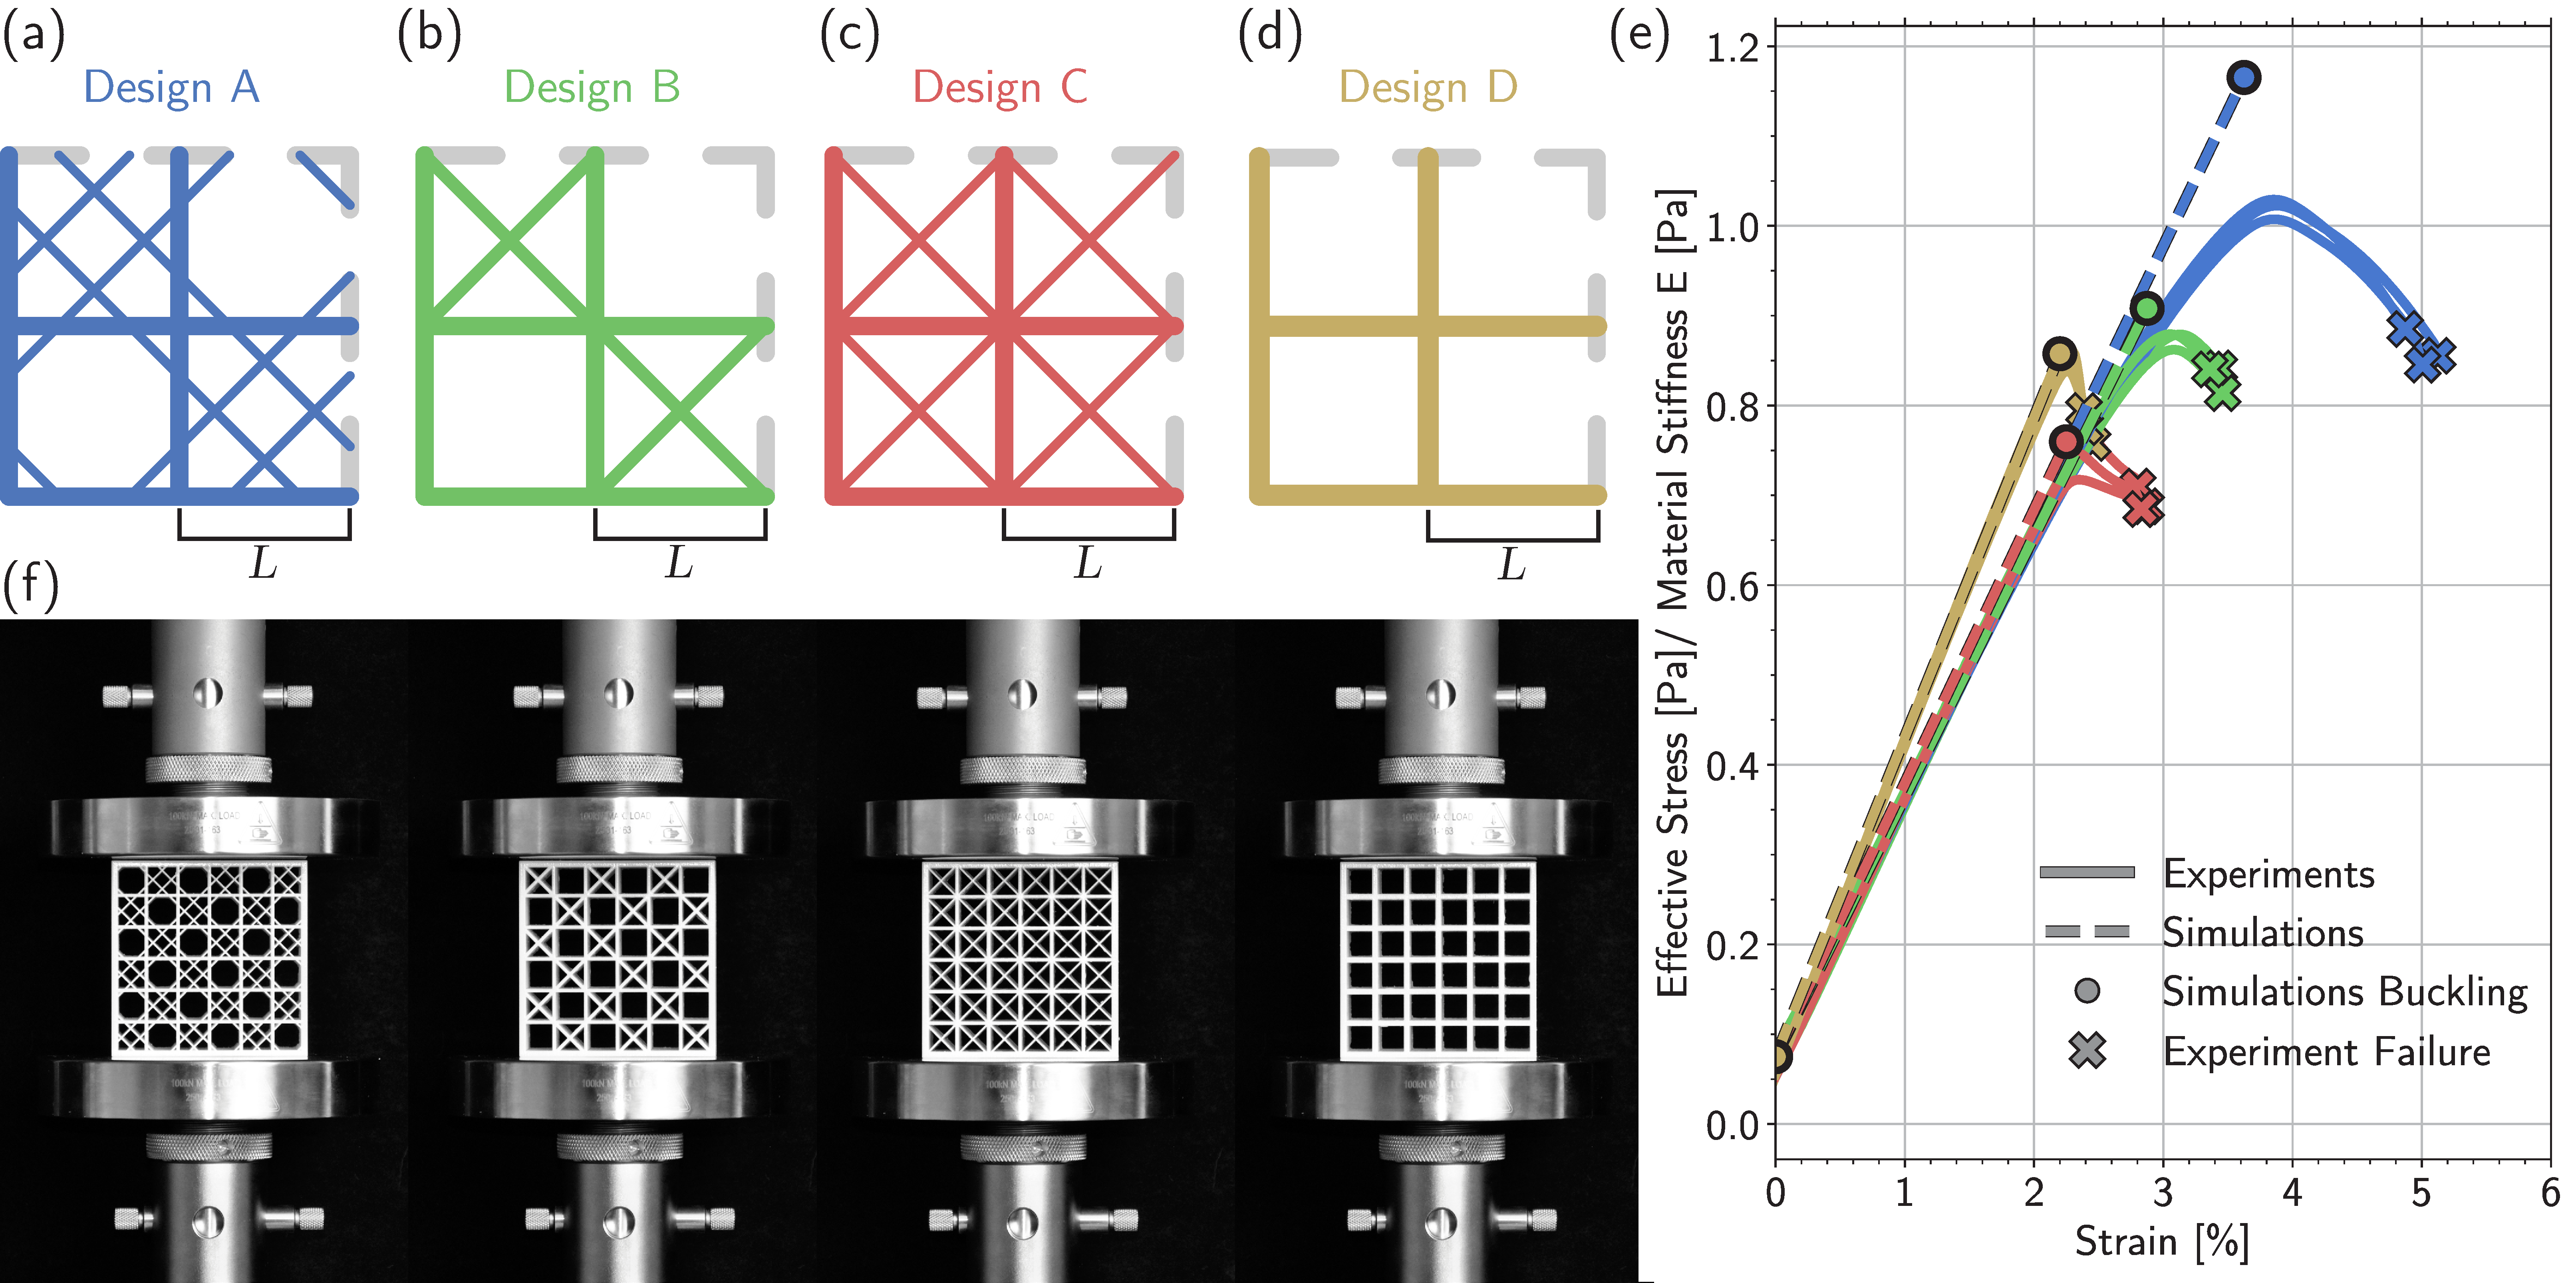
\includegraphics[width=0.9\textwidth]{Fig2}
	\caption{text}\label{Fig2}
\end{figure*}

\begin{figure*}[ht]
	\captionsetup{width=0.8\textwidth}
	\begin{center}
		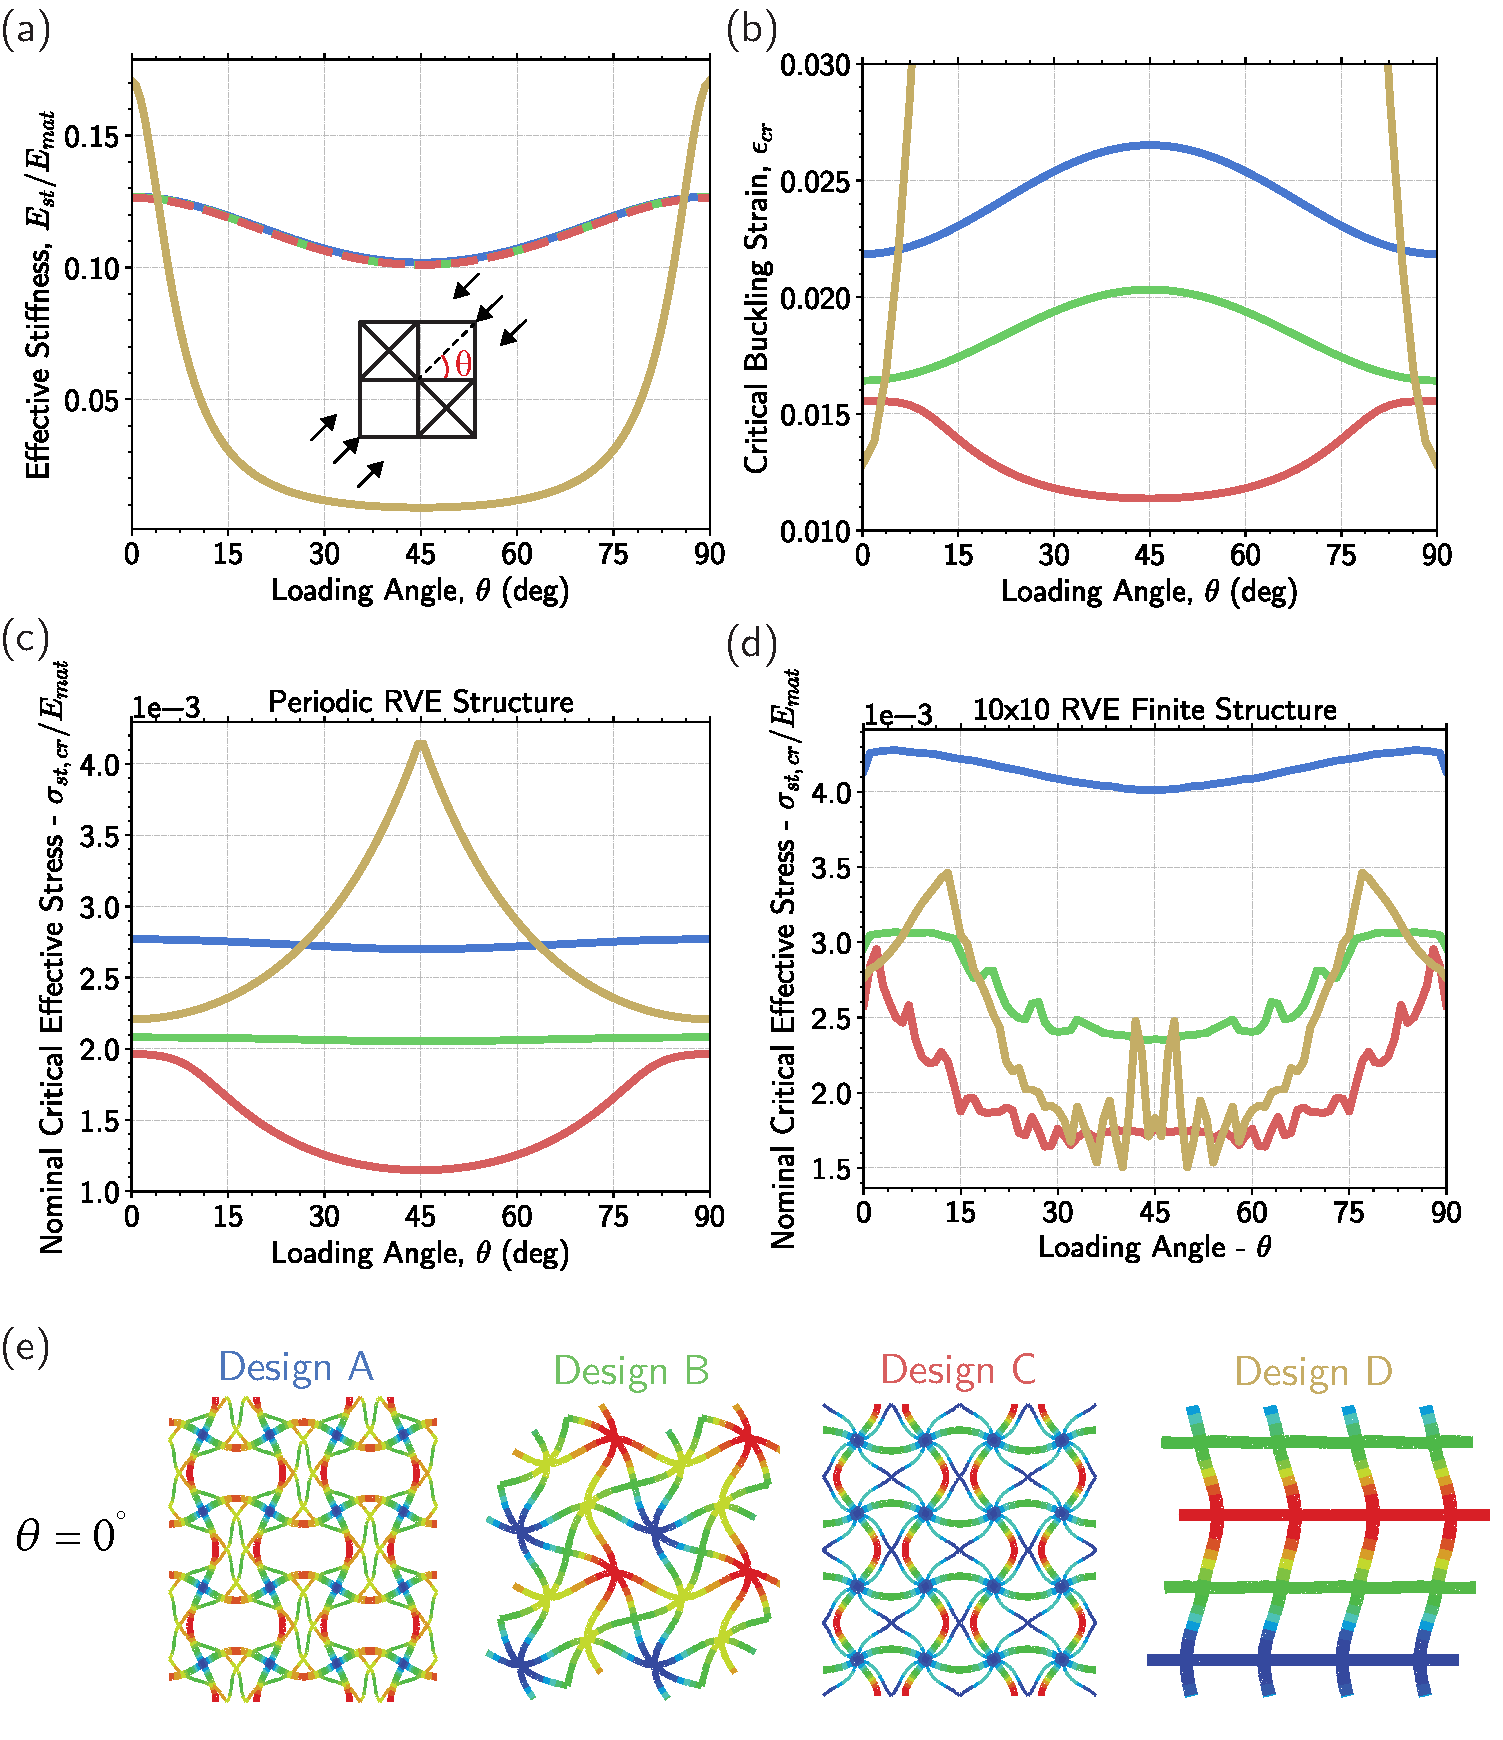
\includegraphics[width=0.7\textwidth]{Fig3}
	\end{center}
	\caption{\textbf{text} Figure showing (a) the structural stiffness for the different designs and (b) the buckling resistance for the different designs. The designs considered are depicted below as Design A-D.} \label{Fig3}
\end{figure*}




% \section{Introduction}
The foundational structure of diagonal reinforcement for truss systems found in bridges, buildings, and beam structures has not changed much since the introduction of the Long truss design patented by Colonel Long in 1830 \citep{waddell1916}. In modern day structures, we see many different iterations of new truss designs with various applications in mind but with what is the same fundamentally simple diagonal reinforcement technique. This technique, involving two diagonal trusses (one in each direction) crossing the opening of a square beam cell, limits the transverse motion of the main support beams ultimately giving the structure shear capacity and strength. Alternative, methods to strengthen beam structures have been introduced via material \hl{[...],} \mf{needs more information and citations}. However, in this study we seek to further strengthen square lattices through inspiration from a particular sponge species called \textit{Euplectella Aspergillum}, commonly known as the Venus' flower basket. This particular species, which is part of the \textit{Hexactinellid} class, is primarily made of silica and exhibit a periodic and regular grid structure with an intrinsic and different diagonal reinforcement scheme. 

Hexactinellids, also known as glass sponges, are predominately deep sea sponges that live in ocean depths of 100-2000m. Beyond their fracture propagation inhibiting material composition \citep{weaver2007}, they are perceived to exhibit large structural rigidity and strength against buckling. 
% Since they are primarily made of 'brittle silica', buckling strength may be a crucial property in making them resistant to impact and environmentally applied stresses. 
Structurally, they are composed of a base square-grid architecture and regular ordering of vertical and horizontal struts that form the skeletal system. Furthermore, their base structure is overlaid with double diagonal (two diagonals in each direction) reinforcement struts, which create a checkerboard-like pattern of open-closed cell structure. This diagonal reinforcement design is conjectured to give the sponge greater buckling resistance and strength to localized damage then it would experience having a single diagonal reinforcement strut (with equivalent allocation of mass between the diagonal reinforcements.) 
% Analogous to the sponge, many engineering structures, such as buildings and bridges, exhibit diagonal reinforcement struts as a stability mechanism. Based on this similarity, we explore the following research question:
The similarity in the structures of the sponge architecture and what we see in the Long truss design has inspired us to further explore the following research question: \textbf{Can we generate design principles for diagonal reinforcements of square beam lattices that are optimally designed to avoid global and/or local structural buckling?} \mf{this paragraph needs more citations and more avid lit. survey}

In this paper, we present a numerical analysis of the structure deformation under various loading conditions as well as survey different arrangements within similar design space of the sponge via parametric studies. Through the various design iterations we look for the critical buckling strain and the elastic load carrying capacity. Finally, we compare the results obtained from the sponge design to what is typically used in engineering structures and validate our results with experimental data.

% involving the development of truss structures with efficient diagonal reinforcement, is inspired by glass sponges (primarily made of silica) commonly known as the Venus Flower Basket. These deep sea sponges exhibit a regular and periodic truss structure which biologists for many years have stipulated to be an optimized design for structural and hydrodynamic purposes. To investigate these claims, I have built numerical and analytical models analyzing the buckling effects of the sponge designs by tuning various geometrical parameters and analyzing its effect on the buckling response. Thus far, we have found the the double diagonal reinforced sponge design delays the onset of structural buckling by a factor of twice the applied strain in comparison to the traditional designs. We believe that this intricate approach inspired by the sponge can improve the way we construct buildings and bridges, which will give the opportunity to build taller buildings and bridges that use less material and are stronger. 

% \section{Results}
% \subsection{Linear Stiffness for different Designs}
In this section, we compare the linear stiffness for the different arrangements using Finite Element Analysis (FEA). For each design, we consider a Representative Volume Element (RVE) and apply periodic boundary conditions along the edges of the unit cell domains depicted along the bottom of \cref{Fig3}. In our numerical model we assume Timoshenko beam elements with uniform circular cross-sections and pin-joints at beam intersections. In an effort to create a method for impartial comparison, we maintain a constant total mass (or constant volume as the material is assumed to be incompressible) between all of the designs, as well as a constant mass ratio between diagonal and non-diagonal elements for designs containing these diagonal reinforcement. 

The results presented in \cref{Fig3}(a) show that all of the structures containing diagonal reinforcement behave the same way for varying loading angles. This illustrates the fact that the structural stiffness is independent of design, but instead depend on the amount of material allocated to the perpendicular aligned beam elements. This is further supported by the graph for Design D, where all of the material from the diagonal beams is removed and allocated to the non-diagonal elements, giving the structure a higher stiffness at $0^\circ$ and lower stiffness at $45^\circ$. Any stiffness at $45^\circ$ in Design D is strictly a result of the bending resistance due to the pinned joints between the non-diagonal beams.

% \subsection{Buckling Resistance for Different Designs}
The results shown in \cref{Fig3}(b) indicate that the structural buckling strength is clearly dependent on the design and alignment of the beam elements. From this figure, we can see that Design A, the sponge design, has the highest buckling strength compared to the other designs containing diagonal reinforcement. At $45^\circ$ loading, Design A improves the buckling strength by a factor of 2.5 times that of Design C, which is the commonly used truss systems. 

% \subsection{Experimental Validation}
For the experimental validation, we conducted various uniaxial compression tests of 3D printed planar beam structures (with circular cross-section) on an Instron 5566. The specimen was 3D printed using \hl{xxxx} material with manufacturer reported \hl{xxxx GPa} modulus. The printed specimen consisted of a 10x10 cell structure spanning a total of 10x10 inch planar structure. The experimental set-up consisted of two \hl{1 inch} thickness acrylic sheets bolted together along the perimeter and spaced from each other by the thickness of the 3D printed specimen.\\\\\hl{[...]} \mf{more to go here when we have experimental setup and data}


% \figll{Buckling_Separation}{0.9}{Critical buckling strain for varying diagonal separation in Design A parametric sweep. The normalized separation distance $C/L$ indicates how far apart the diagonals are from each other. For $C/L=0$ we obtain the Design B and for $C/L=0.5$ we obtain the diagonals crossing half way through the length of the non-diagonal trusses ($L$). For all values in this sweep, we assume a mass ratio equivalent to that of the sponge. The dashed gray line indicates the assumed diagonal separation of the sponge of $C/L=1/(\sqrt{2}+2)$.}

In order to study the impact of diagonal separation for Design A (sponge design), we perform a parametric study on the buckling behavior of the structure under varying separation distances ($C$). Note, we do not perform a stiffness test as the linear stiffness is not dependent on design but instead depends on the mass ratio between diagonal and non-diagonal elements as well as the diagonal element's angles. \Cref{Fig5}(a) shows the buckling behavior as a function of the non-dimensional separation ($C/L$). Where at $C/L=0$ we obtain Design B, and at $C/L=0.5$ we obtain diamond shaped reinforcement alignment. 

% \section{Mass Ratio Parametrization}
% \figll{Stiffness_MassRatio}{0.9}{Structural stiffness for varying mass ratio parametric sweep. Mass ratio $\lambda$ indicates how much mass is allocated to the diagonal elements and non-diagonal elements. For all values in this graph, the design is kept constant while the cross-sectional area of each element is scaled accordingly. For all values of $\lambda$, the total mass of all elements are kept constant. The different colored lines correspond to different loading angles of the unit cell. The gray dashed line indicates the measured mass ratio for the sponge. For all values of this sweep, we assume Design A geometry although the linear stiffness does not depend on the design.}

% \figll{Buckling_MassRatio}{0.9}{Critical buckling strain for varying mass ratio parametric sweep. Mass ratio $\lambda$ indicates how much mass is allocated to the diagonal elements and non-diagonal elements. For all values in this graph, the design is kept constant while the cross-sectional area of each element is scaled accordingly. For all values of $\lambda$, the total mass of all elements are kept constant. The different colored lines correspond to different loading angles of the unit cell. The gray dashed line indicates the measured mass ratio for the sponge. For all values of this sweep, we assume Design A geometry.}

% \section{Diagonal Separation Parametrization}

To investigate the effect of mass ratio on the properties of the structure, we parametrize the allocation of mass between the diagonal elements and the non-diagonal elements. To quantitatively describe this mass ratio, we introduce the variable $\lambda$ as the fraction $V_{nd}/V_d$, where $V_{nd}$ describes the collective volume of all non-diagonal elements and $V_d$ is the collective volume of all diagonal elements in the unit cell. It is important to note, that for all simulations varying $\lambda$ we maintain the same total mass of the structure, namely $V_{nd}+V_d=\mbox{const. } \forall (V_{nd},V_d)$. 

\Cref{Fig5}(b) shows the structural stiffness as a function of $\lambda$ for various loading angles (corresponding to the respective colors). In this figure, we see that for small $\lambda$ the structure is stiffer at $0^\circ$ loading and for large $\lambda$ the structure is stiffer at $45^\circ$. This is expected as we are allocating more material to its respective elements. Furthermore, we can see that at $\lambda=1$ we attain a point in the mass ratio where the stiffness is equal for all angles. That is because there is the same amount of material allocated to the diagonals as there is to the non-diagonal elements.

\Cref{Fig5}(c) illustrates the critical buckling strain as a function of $\lambda$. Here, we can clearly see that buckling strain is dependent on the mass ratio and behaves differently for all angles \hl{[...]} \mf{I am not sure what to say here (interpretation) about this graph.}


% \section{Conclusion}
% \hl{add writing}

\section*{Funding Information}
\hl{add writing}
% No. NSF-GRFP DGE-1144152 (for M. C. F.), GEM Consortium Fellowship

\section*{Acknowledgments}
\hl{add writing} 
% Wyss Institute for equipment. James R. Rice. Mark Scott. Joanna Aizenberg. Joost Vlassak. Chris Rycroft




%\begin{figure*}
%	\captionsetup{width=0.8\textwidth}
%	\begin{center}
%		\includegraphics[width=0.7\textwidth]{Fig5}
%	\end{center}
%	\caption{\textbf{Parametric sweep results for different analysis.} (a) Critical buckling strain for varying diagonal separation in Design A. The normalized separation distance $C/L$ indicates how far apart the diagonals are from each other. For all values we assume a mass ratio to be equivalent to that of the sponge. The dashed gray line indicates the assumed diagonal separation of the sponge, namely $C/L=1/(\sqrt{2}+2)$. (b) Structural linear stiffness for varying mass ratio. Mass ratio $\lambda$ indicates how much mass is allocated to the diagonal elements and non-diagonal elements based on the volume element. For all values of $\lambda$, the total mass of all elements are kept constant. The gray dashed line indicates the measured mass ratio for the sponge. (c) Critical buckling strain for varying mass ratio. For all values of $\lambda$, the total mass of all elements are kept constant. The different colored lines correspond to different loading angles of the unit cell. The gray dashed line indicates the measured mass ratio for the sponge. For all values in (b) and (c), we assume Design A geometry.} \label{Fig5}
%\end{figure*}

 Bibliography
\nocite{*}
\bibliography{refs}
\bibliographystyle{apalike}




\end{document}